% Capitolul 10: Recapitulare Completă - Complete Time Series Analysis
% Applying all methods to real data: Bitcoin, Sunspots, Unemployment
% Bachelor program, Bucharest University of Economic Studies

\documentclass[9pt, aspectratio=169, t]{beamer}

% Ensure content fits on slides
\setbeamersize{text margin left=8mm, text margin right=8mm}

%=============================================================================
% THEME AND STYLE CONFIGURATION
%=============================================================================
\usetheme{Madrid}
\usecolortheme{seahorse}

% IDA-Inspired Color Palette
\definecolor{MainBlue}{RGB}{26, 58, 110}
\definecolor{AccentBlue}{RGB}{42, 82, 140}
\definecolor{IDAred}{RGB}{220, 53, 69}
\definecolor{DarkGray}{RGB}{51, 51, 51}
\definecolor{MediumGray}{RGB}{128, 128, 128}
\definecolor{LightGray}{RGB}{248, 248, 248}
\definecolor{VeryLightGray}{RGB}{235, 235, 235}
\definecolor{Crimson}{RGB}{220, 53, 69}
\definecolor{Forest}{RGB}{46, 125, 50}
\definecolor{Amber}{RGB}{181, 133, 63}
\definecolor{Orange}{RGB}{230, 126, 34}
\definecolor{BitcoinOrange}{RGB}{247, 147, 26}

\setbeamercolor{palette primary}{bg=MainBlue, fg=white}
\setbeamercolor{palette secondary}{bg=MainBlue!85, fg=white}
\setbeamercolor{palette tertiary}{bg=MainBlue!70, fg=white}
\setbeamercolor{structure}{fg=MainBlue}
\setbeamercolor{title}{fg=MainBlue}
\setbeamercolor{frametitle}{fg=MainBlue, bg=white}
\setbeamercolor{block title}{bg=MainBlue, fg=white}
\setbeamercolor{block body}{bg=VeryLightGray, fg=DarkGray}
\setbeamercolor{block title alerted}{bg=Crimson, fg=white}
\setbeamercolor{block body alerted}{bg=Crimson!8, fg=DarkGray}
\setbeamercolor{block title example}{bg=Forest, fg=white}
\setbeamercolor{block body example}{bg=Forest!8, fg=DarkGray}
\setbeamercolor{item}{fg=MainBlue}

\setbeamertemplate{navigation symbols}{}

\setbeamertemplate{footline}{
    \leavevmode%
    \hbox{%
        \begin{beamercolorbox}[wd=.333333\paperwidth,ht=2.5ex,dp=1ex,center]{author in head/foot}%
            \usebeamerfont{author in head/foot}\insertshortauthor
        \end{beamercolorbox}%
        \begin{beamercolorbox}[wd=.333333\paperwidth,ht=2.5ex,dp=1ex,center]{title in head/foot}%
            \usebeamerfont{title in head/foot}\insertshorttitle
        \end{beamercolorbox}%
        \begin{beamercolorbox}[wd=.333333\paperwidth,ht=2.5ex,dp=1ex,right]{date in head/foot}%
            \usebeamerfont{date in head/foot}\insertshortdate{}\hspace*{2em}
            \insertframenumber{} / \inserttotalframenumber\hspace*{2ex}
        \end{beamercolorbox}}%
    \vskip0pt%
}

%=============================================================================
% PACKAGES
%=============================================================================
\usepackage[utf8]{inputenc}
\usepackage[T1]{fontenc}
\usepackage{amsmath, amssymb, amsthm}
\usepackage{mathtools}
\usepackage{bm}
\usepackage{tikz}
\usetikzlibrary{arrows.meta, positioning, shapes, calc}
\usepackage{booktabs}
\usepackage{multirow}
\usepackage{array}
\usepackage{graphicx}
\usepackage{hyperref}
\hypersetup{colorlinks=false, pdfborder={0 0 0}}
\graphicspath{{../logos/}{../charts/}}

%=============================================================================
% THEOREM ENVIRONMENTS
%=============================================================================
\theoremstyle{definition}
\setbeamertemplate{theorems}[numbered]
\newtheorem{defn}{Definition}
\newtheorem{thm}{Theorem}
\newtheorem{prop}{Proposition}

%=============================================================================
% CUSTOM COMMANDS
%=============================================================================
\newcommand{\E}{\mathbb{E}}
\newcommand{\Var}{\text{Var}}
\newcommand{\Cov}{\text{Cov}}
\newcommand{\Corr}{\text{Corr}}
\newcommand{\R}{\mathbb{R}}

%=============================================================================
% TITLE INFORMATION
%=============================================================================
\title[Capitolul 10: Recapitulare Completă]{Capitolul 10: Recapitulare Completă}
\subtitle{Bachelor Program, Faculty of Cybernetics, Statistics and Economic Informatics, Bucharest University of Economic Studies}
\author[Prof. Daniel Traian Pele, PhD]{Prof. Daniel Traian Pele, PhD\\[0.2cm]\footnotesize\texttt{danpele@ase.ro}}
\institute{Bucharest University of Economic Studies}
\date{Academic Year 2025--2026}

\begin{document}

%=============================================================================
% TITLE SLIDE
%=============================================================================
\begin{frame}[plain]
    \begin{tikzpicture}[remember picture, overlay]
        \fill[IDAred] (current page.north west) rectangle ([yshift=-0.15cm]current page.north east);
        \node[anchor=north west] at ([xshift=0.5cm, yshift=-0.3cm]current page.north west) {
            \href{https://www.ase.ro}{\includegraphics[height=1.1cm]{ase_logo.png}}
        };
        \node[anchor=north] at ([yshift=-0.3cm]current page.north) {
            \href{https://ai4efin.ase.ro}{\includegraphics[height=1.1cm]{ai4efin_logo.png}}
        };
        \node[anchor=north east] at ([xshift=-0.5cm, yshift=-0.3cm]current page.north east) {
            \href{https://www.digital-finance-msca.com}{\includegraphics[height=1.1cm]{msca_logo.png}}
        };
    \end{tikzpicture}
    \vfill
    \begin{center}
        {\Large\textcolor{MediumGray}{Analiza și Prognoza Seriilor de Timp}}\\[0.3cm]
        {\Huge\textbf{\textcolor{MainBlue}{Capitolul 10: Recapitulare Completă}}}\\[0.5cm]
        {\Large\textcolor{IDAred}{Analiză Completă cu Date Reale}}
    \end{center}
    \vfill

    \begin{tikzpicture}[remember picture, overlay]
        \fill[IDAred] (current page.south west) rectangle ([yshift=0.15cm]current page.south east);
        \node[anchor=south west] at ([xshift=0.5cm, yshift=0.8cm]current page.south west) {
            \href{https://theida.net}{\includegraphics[height=0.9cm]{ida_logo.png}}
        };
        \node[anchor=south] at ([xshift=-3cm, yshift=0.8cm]current page.south) {
            \href{https://blockchain-research-center.com}{\includegraphics[height=0.9cm]{brc_logo.png}}
        };
        \node[anchor=south] at ([yshift=0.8cm]current page.south) {
            \href{https://quantinar.com}{\includegraphics[height=0.9cm]{qr_logo.png}}
        };
        \node[anchor=south] at ([xshift=3cm, yshift=0.8cm]current page.south) {
            \href{https://quantlet.com}{\includegraphics[height=0.9cm]{ql_logo.png}}
        };
        \node[anchor=south east] at ([xshift=-0.5cm, yshift=0.8cm]current page.south east) {
            \href{https://ipe.ro/new}{\includegraphics[height=0.9cm]{acad_logo.png}}
        };
    \end{tikzpicture}
\end{frame}

%=============================================================================
% TABLE OF CONTENTS
%=============================================================================
\begin{frame}{Cuprins}
    \tableofcontents
\end{frame}

%=============================================================================
% SECTION 1: INTRODUCTION
%=============================================================================
\section{Fluxul Complet de Analiză}

\begin{frame}{Prezentare Generală: Metode Studiate}
    \begin{columns}[T]
        \begin{column}{0.48\textwidth}
            \textbf{Metode Clasice}
            \begin{itemize}
                \item \textcolor{MainBlue}{Cap 1:} Fundamentele Seriilor de Timp
                \item \textcolor{MainBlue}{Cap 2:} Modele ARMA
                \item \textcolor{MainBlue}{Cap 3:} Modele ARIMA
                \item \textcolor{MainBlue}{Cap 4:} Modele SARIMA
                \item \textcolor{MainBlue}{Cap 5:} Modele GARCH
            \end{itemize}
        \end{column}
        \begin{column}{0.48\textwidth}
            \textbf{Metode Avansate}
            \begin{itemize}
                \item \textcolor{Forest}{Cap 6:} VAR \& Cauzalitate Granger
                \item \textcolor{Forest}{Cap 7:} Cointegrare \& VECM
                \item \textcolor{Forest}{Cap 8:} Extensii Moderne
                \item \textcolor{Forest}{Cap 9:} Prophet \& TBATS
            \end{itemize}
            \vspace{0.5em}
            \textbf{Astăzi: Aplicăm TOATE pe Date Reale!}
        \end{column}
    \end{columns}
\end{frame}

\begin{frame}{Fluxul Complet de Analiză}
    \begin{center}
        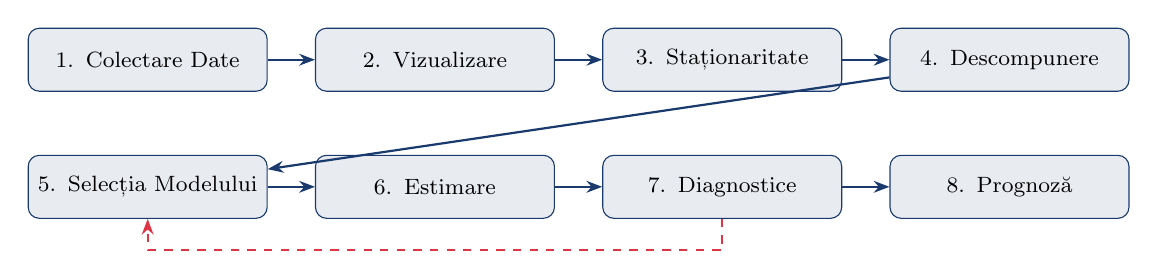
\begin{tikzpicture}[
            node distance=0.6cm,
            box/.style={rectangle, rounded corners, draw=MainBlue, fill=MainBlue!10,
                        text width=2.8cm, minimum height=0.8cm, align=center, font=\footnotesize},
            arrow/.style={-{Stealth[length=2mm]}, thick, MainBlue}
        ]
            % Row 1
            \node[box] (data) {1. Colectare Date};
            \node[box, right=of data] (viz) {2. Vizualizare};
            \node[box, right=of viz] (stat) {3. Staționaritate};
            \node[box, right=of stat] (decomp) {4. Descompunere};

            % Row 2
            \node[box, below=0.8cm of data] (model) {5. Selecția Modelului};
            \node[box, right=of model] (est) {6. Estimare};
            \node[box, right=of est] (diag) {7. Diagnostice};
            \node[box, right=of diag] (forecast) {8. Prognoză};

            % Arrows
            \draw[arrow] (data) -- (viz);
            \draw[arrow] (viz) -- (stat);
            \draw[arrow] (stat) -- (decomp);
            \draw[arrow] (decomp) -- (model);
            \draw[arrow] (model) -- (est);
            \draw[arrow] (est) -- (diag);
            \draw[arrow] (diag) -- (forecast);

            % Feedback loop
            \draw[arrow, dashed, IDAred] (diag.south) -- ++(0,-0.4) -| (model.south);
        \end{tikzpicture}
    \end{center}

    \vspace{0.3cm}
    \begin{alertblock}{Principiu Cheie}
        Diagnosticele pot necesita revenirea la selecția modelului (proces iterativ)
    \end{alertblock}
\end{frame}

\begin{frame}{Seturi de Date Reale pentru Acest Capitol}
    \begin{columns}[T]
        \begin{column}{0.24\textwidth}
            \begin{block}{\textcolor{BitcoinOrange}{Bitcoin}}
                \begin{itemize}
                    \item Zilnic 2019-2024
                    \item Clustering volatilitate
                    \item ARIMA + GARCH
                \end{itemize}
            \end{block}
        \end{column}
        \begin{column}{0.24\textwidth}
            \begin{block}{\textcolor{Orange}{Pete Solare}}
                \begin{itemize}
                    \item Anual 1900-2023
                    \item Ciclu de 11 ani
                    \item Termeni Fourier
                \end{itemize}
            \end{block}
        \end{column}
        \begin{column}{0.24\textwidth}
            \begin{block}{\textcolor{MainBlue}{Șomaj}}
                \begin{itemize}
                    \item Lunar 2010-2023
                    \item Șocul COVID-19
                    \item Prophet
                \end{itemize}
            \end{block}
        \end{column}
        \begin{column}{0.24\textwidth}
            \begin{block}{\textcolor{Forest}{Economic VAR}}
                \begin{itemize}
                    \item Trimestrial 2000-2023
                    \item PIB, Inflație, etc.
                    \item VAR Multivariat
                \end{itemize}
            \end{block}
        \end{column}
    \end{columns}
\end{frame}

%=============================================================================
% SECTION 2: CASE STUDY 1 - BITCOIN
%=============================================================================
\section{Studiu de Caz 1: Analiza Volatilității Bitcoin}

\begin{frame}{Bitcoin: Prezentare Generală a Datelor}
    \begin{center}
        \includegraphics[width=0.95\textwidth, height=0.70\textheight, keepaspectratio]{ch10_bitcoin_overview.pdf}
    \end{center}

    \begin{itemize}
        \item \textbf{Date:} Prețuri zilnice Bitcoin și randamente logaritmice (2019-2024)
        \item \textbf{Evenimente cheie:} Crahul COVID, bull run 2021, iarna crypto 2022
    \end{itemize}
\end{frame}

\begin{frame}{Pasul 1: Testarea Staționarității}
    \begin{columns}[T]
        \begin{column}{0.55\textwidth}
            \textbf{Testul Augmented Dickey-Fuller}
            \begin{itemize}
                \item $H_0$: Rădăcină unitară (nestaționară)
                \item $H_1$: Staționară
            \end{itemize}

            \vspace{0.5em}
            \textbf{Rezultate pentru Bitcoin:}
            \begin{table}[h]
                \footnotesize
                \begin{tabular}{lcc}
                    \toprule
                    Serie & Statistică ADF & p-value \\
                    \midrule
                    Prețuri & $-0.87$ & 0.79 \\
                    Randamente Log & $-42.1$ & $<0.001$ \\
                    \bottomrule
                \end{tabular}
            \end{table}

            \vspace{0.5em}
            $\Rightarrow$ Prețuri: nestaționare (random walk) \\
            $\Rightarrow$ Randamente: staționare
        \end{column}
        \begin{column}{0.43\textwidth}
            \begin{exampleblock}{Testul KPSS (Confirmare)}
                \begin{itemize}
                    \item $H_0$: Staționară
                    \item $H_1$: Rădăcină unitară
                \end{itemize}

                \vspace{0.3em}
                Prețuri: KPSS = 5.83** \\
                Randamente: KPSS = 0.12

                \vspace{0.3em}
                \textcolor{Forest}{Ambele teste confirmă: folosim randamente log!}
            \end{exampleblock}
        \end{column}
    \end{columns}
\end{frame}

\begin{frame}{Pasul 2: Analiza ACF/PACF a Randamentelor}
    \begin{center}
        \includegraphics[width=0.95\textwidth, height=0.65\textheight, keepaspectratio]{ch10_bitcoin_acf_pacf.pdf}
    \end{center}

    \begin{itemize}
        \item \textbf{Randamente:} Aproape zgomot alb (dependență liniară slabă)
        \item \textbf{Randamente pătratice:} Persistență puternică $\Rightarrow$ \textcolor{IDAred}{clustering volatilitate}
        \item \textbf{Implicație:} Modelul GARCH este esențial pentru Bitcoin!
    \end{itemize}
\end{frame}

\begin{frame}{Pasul 3: Model ARIMA pentru Randamente}
    \textbf{Selecția Modelului folosind AIC/BIC:}

    \begin{columns}[T]
        \begin{column}{0.48\textwidth}
            \begin{table}[h]
                \footnotesize
                \begin{tabular}{lcc}
                    \toprule
                    Model & AIC & BIC \\
                    \midrule
                    ARIMA(0,0,0) & 9524 & 9530 \\
                    ARIMA(1,0,0) & 9522 & 9534 \\
                    ARIMA(0,0,1) & 9523 & 9535 \\
                    \textbf{ARIMA(1,0,1)} & \textbf{9520} & \textbf{9538} \\
                    \bottomrule
                \end{tabular}
            \end{table}

            \vspace{0.3em}
            Cel mai bun: ARIMA(1,0,1) dar îmbunătățire marginală
        \end{column}
        \begin{column}{0.48\textwidth}
            \begin{alertblock}{Observație Cheie}
                Randamentele crypto sunt notoriu imprevizibile. ``Alpha'' este în înțelegerea \textbf{dinamicii volatilității}, nu în predicția direcției!
            \end{alertblock}
        \end{column}
    \end{columns}
\end{frame}

\begin{frame}{Pasul 4: Model GARCH pentru Volatilitate}
    \begin{center}
        \includegraphics[width=0.95\textwidth, height=0.60\textheight, keepaspectratio]{ch10_bitcoin_garch.pdf}
    \end{center}

    \textbf{Modelul GARCH(1,1):}
    \[
        \sigma_t^2 = \omega + \alpha \varepsilon_{t-1}^2 + \beta \sigma_{t-1}^2
    \]

    \begin{itemize}
        \item Bitcoin arată $\alpha + \beta \approx 0.95$ (persistență ridicată)
        \item Perioadele COVID și Mai 2021 arată vârfuri masive de volatilitate
    \end{itemize}
\end{frame}

\begin{frame}{Bitcoin: Rezumatul Abordării}
    \begin{center}
        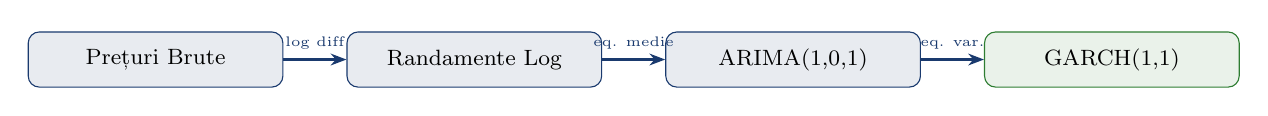
\begin{tikzpicture}[
            node distance=0.4cm,
            box/.style={rectangle, rounded corners, draw=MainBlue, fill=MainBlue!10,
                        text width=3cm, minimum height=0.7cm, align=center, font=\footnotesize},
            result/.style={rectangle, rounded corners, draw=Forest, fill=Forest!10,
                          text width=3cm, minimum height=0.7cm, align=center, font=\footnotesize},
            arrow/.style={-{Stealth[length=2mm]}, thick, MainBlue}
        ]
            \node[box] (prices) {Prețuri Brute};
            \node[box, right=0.8cm of prices] (returns) {Randamente Log};
            \node[box, right=0.8cm of returns] (arima) {ARIMA(1,0,1)};
            \node[result, right=0.8cm of arima] (garch) {GARCH(1,1)};

            \draw[arrow] (prices) -- node[above, font=\tiny] {log diff} (returns);
            \draw[arrow] (returns) -- node[above, font=\tiny] {eq. medie} (arima);
            \draw[arrow] (arima) -- node[above, font=\tiny] {eq. var.} (garch);
        \end{tikzpicture}
    \end{center}

    \vspace{0.5em}
    \begin{columns}[T]
        \begin{column}{0.48\textwidth}
            \textbf{Constatări Cheie:}
            \begin{itemize}
                \item Randamentele sunt aproape imprevizibile
                \item Clustering extrem de volatilitate
                \item GARCH captează dinamica riscului
            \end{itemize}
        \end{column}
        \begin{column}{0.48\textwidth}
            \textbf{Utilizare Practică:}
            \begin{itemize}
                \item Managementul riscului (VaR, CVaR)
                \item Dimensionarea pozițiilor
                \item Strategii de trading pe volatilitate
            \end{itemize}
        \end{column}
    \end{columns}
\end{frame}

%=============================================================================
% SECTION 3: CASE STUDY 2 - SUNSPOTS
%=============================================================================
\section{Studiu de Caz 2: Analiza Ciclului Petelor Solare}

\begin{frame}{Pete Solare: Un Set de Date Clasic cu Ciclu Lung}
    \begin{center}
        \includegraphics[width=0.95\textwidth, height=0.65\textheight, keepaspectratio]{ch10_sunspot_overview.pdf}
    \end{center}

    \begin{itemize}
        \item \textbf{Date:} Numere lunare de pete solare, 1990-2023
        \item \textbf{Caracteristici:} Celebrul ciclu solar de $\sim$11 ani (132 luni)
    \end{itemize}
\end{frame}

\begin{frame}{Pasul 1: Analiza Descompunerii}
    \begin{center}
        \includegraphics[width=0.95\textwidth, height=0.65\textheight, keepaspectratio]{ch10_sunspot_decomposition.pdf}
    \end{center}

    \begin{itemize}
        \item \textbf{Trend:} Media pe termen lung a activității solare
        \item \textbf{Ciclu:} Ciclul solar de 11 ani (ciclul Schwabe)
        \item \textbf{Provocare:} Perioadă sezonieră foarte lungă ($m = 132$)
    \end{itemize}
\end{frame}

\begin{frame}{Pasul 2: Gestionarea Sezonalității Lungi}
    \textbf{Provocarea:}
    \begin{itemize}
        \item SARIMA standard cu $m=132$ necesită estimarea multor parametri
        \item Diferențierea sezonieră la lag 132 pierde 11 ani de date!
    \end{itemize}

    \vspace{0.5em}
    \begin{columns}[T]
        \begin{column}{0.48\textwidth}
            \textbf{Opțiunea 1: Termeni Fourier}
            \begin{itemize}
                \item Adăugăm regresori sinus/cosinus
                \item Perioadă = 132 luni
                \item Mai puțini parametri decât SARIMA complet
            \end{itemize}

            \[
                \sum_{k=1}^{K} \left[ a_k \sin\left(\frac{2\pi k t}{132}\right) + b_k \cos\left(\frac{2\pi k t}{132}\right) \right]
            \]
        \end{column}
        \begin{column}{0.48\textwidth}
            \textbf{Opțiunea 2: Model AR}
            \begin{itemize}
                \item AR de ordin înalt captează ciclul
                \item AR(12) sau AR(24) adesea suficient
                \item Simplu și eficient
            \end{itemize}

            \vspace{0.5em}
            \begin{exampleblock}{Rezultat Clasic}
                Petele solare sunt bine modelate de modele AR(9) sau AR(12) (Yule, 1927)
            \end{exampleblock}
        \end{column}
    \end{columns}
\end{frame}

\begin{frame}{Pasul 3: Prognoza SARIMA}
    \begin{center}
        \includegraphics[width=0.95\textwidth, height=0.60\textheight, keepaspectratio]{ch10_sunspot_sarima.pdf}
    \end{center}

    \textbf{Model:} AR(12) cu termeni Fourier pentru ciclul de 11 ani

    \begin{itemize}
        \item Captează comportamentul cvasi-periodic
        \item Incertitudinea prognozei crește semnificativ cu orizontul
    \end{itemize}
\end{frame}

\begin{frame}{Pete Solare: Comparația Modelelor}
    \begin{table}[h]
        \footnotesize
        \centering
        \begin{tabular}{lccc}
            \toprule
            Model & RMSE & MAE & Note \\
            \midrule
            AR(12) & 28.4 & 22.1 & Simplu, interpretabil \\
            ARIMA(2,0,2) + Fourier & 26.8 & 20.5 & Captură bună a ciclului \\
            \textbf{TBATS} & \textbf{25.2} & \textbf{19.8} & Detecție automată a ciclului \\
            Prophet & 29.1 & 23.4 & Mai puțin potrivit pentru cicluri lungi \\
            \bottomrule
        \end{tabular}
    \end{table}

    \vspace{0.5em}
    \begin{alertblock}{Lecție Cheie}
        Pentru perioade sezoniere foarte lungi, considerați:
        \begin{itemize}
            \item Termeni de regresie Fourier
            \item TBATS (selecție automată a ciclului)
            \item Modele AR de ordin înalt
        \end{itemize}
    \end{alertblock}
\end{frame}

%=============================================================================
% SECTION 4: CASE STUDY 3 - UNEMPLOYMENT
%=============================================================================
\section{Studiu de Caz 3: Șomajul SUA cu Ruptură Structurală}

\begin{frame}{Șomajul SUA: Șocul COVID-19}
    \begin{center}
        \includegraphics[width=0.95\textwidth, height=0.65\textheight, keepaspectratio]{ch10_unemployment_overview.pdf}
    \end{center}

    \begin{itemize}
        \item \textbf{Date:} Rata Șomajului SUA, lunar, 2015-2023 (BLS)
        \item \textbf{Șoc:} De la 3.5\% la 14.7\% într-o singură lună (Aprilie 2020)!
    \end{itemize}
\end{frame}

\begin{frame}{Gestionarea Rupturilor Structurale}
    \begin{columns}[T]
        \begin{column}{0.48\textwidth}
            \textbf{Opțiunea 1: Trunchierea Datelor}
            \begin{itemize}
                \item Folosim doar date post-COVID
                \item Pro: Curate, fără rupturi
                \item Contra: Pierdem tipare istorice
            \end{itemize}

            \vspace{0.5em}
            \textbf{Opțiunea 2: Variabile Dummy}
            \begin{itemize}
                \item Adăugăm indicator COVID
                \item Pro: Folosește toate datele
                \item Contra: Complex în ARIMA
            \end{itemize}
        \end{column}
        \begin{column}{0.48\textwidth}
            \textbf{Opțiunea 3: Prophet cu Changepoints}
            \begin{itemize}
                \item Detecție automată
                \item Pro: Gestionează rupturile natural
                \item Contra: Poate necesita tuning
            \end{itemize}

            \vspace{0.5em}
            \begin{exampleblock}{Recomandare}
                Pentru date afectate de COVID, detecția changepoint-urilor Prophet sau modelele de schimbare de regim funcționează cel mai bine.
            \end{exampleblock}
        \end{column}
    \end{columns}
\end{frame}

\begin{frame}{Prophet pentru Șomaj}
    \begin{center}
        \includegraphics[width=0.95\textwidth, height=0.60\textheight, keepaspectratio]{ch10_unemployment_prophet.pdf}
    \end{center}

    \textbf{Configurare Prophet:}
    \begin{itemize}
        \item \texttt{changepoint\_prior\_scale = 0.5} (flexibil pentru șocul COVID)
        \item Changepoint automat în Aprilie 2020
        \item Captează tiparul de recuperare în V
    \end{itemize}
\end{frame}

\begin{frame}{Comparația Modelelor pe Șomaj}
    \begin{center}
        \includegraphics[width=0.95\textwidth, height=0.55\textheight, keepaspectratio]{ch10_unemployment_comparison.pdf}
    \end{center}

    \begin{alertblock}{Lecție Cheie}
        Când datele au rupturi structurale extreme:
        \begin{itemize}
            \item ARIMA tradițional poate eșua sau necesită analiză de intervenție
            \item Flexibilitatea Prophet cu changepoints captează schimbările de regim
            \item Considerați modele de schimbare de regim (Markov-switching)
        \end{itemize}
    \end{alertblock}
\end{frame}

%=============================================================================
% SECTION 5: CASE STUDY 4 - VAR MULTIVARIATE
%=============================================================================
\section{Studiu de Caz 4: Analiza Multivariată VAR}

\begin{frame}{De Ce Analiză Multivariată?}
    \begin{columns}[T]
        \begin{column}{0.48\textwidth}
            \textbf{Serie Singulară (Univariată):}
            \begin{itemize}
                \item ARIMA, GARCH, Prophet
                \item O singură variabilă la un moment dat
                \item Nu captează dinamica între serii
            \end{itemize}

            \vspace{0.5em}
            \textbf{Serii Multiple (Multivariate):}
            \begin{itemize}
                \item \textcolor{MainBlue}{VAR}: Vector Autoregression
                \item \textcolor{MainBlue}{VECM}: Cu cointegrare
                \item Captează interdependențele
            \end{itemize}
        \end{column}
        \begin{column}{0.48\textwidth}
            \begin{exampleblock}{Când să Folosim VAR?}
                \begin{itemize}
                    \item Indicatori economici (PIB, inflație, șomaj)
                    \item Piețe financiare (acțiuni, obligațiuni, FX)
                    \item Variabile supply chain
                    \item Orice sistem cu bucle de feedback
                \end{itemize}
            \end{exampleblock}
        \end{column}
    \end{columns}
\end{frame}

\begin{frame}{Modelul VAR: Bazele}
    \textbf{Vector Autoregression VAR(p):}

    Pentru $k$ variabile, VAR(p) este:
    \[
        \mathbf{y}_t = \mathbf{c} + \mathbf{A}_1 \mathbf{y}_{t-1} + \mathbf{A}_2 \mathbf{y}_{t-2} + \cdots + \mathbf{A}_p \mathbf{y}_{t-p} + \boldsymbol{\varepsilon}_t
    \]

    \vspace{0.5em}
    \begin{columns}[T]
        \begin{column}{0.48\textwidth}
            \textbf{Exemplu: VAR(1) cu 2 variabile}
            \[
                \begin{pmatrix} y_{1t} \\ y_{2t} \end{pmatrix} = \begin{pmatrix} c_1 \\ c_2 \end{pmatrix} + \begin{pmatrix} a_{11} & a_{12} \\ a_{21} & a_{22} \end{pmatrix} \begin{pmatrix} y_{1,t-1} \\ y_{2,t-1} \end{pmatrix} + \begin{pmatrix} \varepsilon_{1t} \\ \varepsilon_{2t} \end{pmatrix}
            \]

            \vspace{0.3em}
            \textcolor{IDAred}{Cheie:} Fiecare variabilă depinde de lag-urile TUTUROR variabilelor
        \end{column}
        \begin{column}{0.48\textwidth}
            \textbf{Caracteristici Cheie:}
            \begin{itemize}
                \item Captează feedback dinamic
                \item Toate variabilele sunt endogene
                \item Permite teste de cauzalitate Granger
                \item Analiză impulse response
            \end{itemize}
        \end{column}
    \end{columns}
\end{frame}

\begin{frame}{Studiu de Caz: Variabile Economice SUA}
    \textbf{Variabile (Trimestrial, 2000-2023):}
    \begin{itemize}
        \item \textcolor{MainBlue}{Creștere PIB} (YoY \%)
        \item \textcolor{IDAred}{Rata Șomajului} (\%)
        \item \textcolor{Forest}{Inflație} (CPI YoY \%)
        \item \textcolor{Orange}{Rata Fed Funds} (\%)
    \end{itemize}

    \vspace{0.5em}
    \begin{columns}[T]
        \begin{column}{0.48\textwidth}
            \textbf{Relații Așteptate:}
            \begin{itemize}
                \item PIB $\uparrow$ $\Rightarrow$ Șomaj $\downarrow$ (Legea lui Okun)
                \item PIB $\uparrow$ $\Rightarrow$ Inflație $\uparrow$ (cerere-push)
                \item Inflație $\uparrow$ $\Rightarrow$ Rata Fed $\uparrow$ (Regula Taylor)
            \end{itemize}
        \end{column}
        \begin{column}{0.48\textwidth}
            \textbf{Surse Date (FRED):}
            \begin{itemize}
                \item GDPC1: PIB Real
                \item UNRATE: Șomaj
                \item CPIAUCSL: Indicele Prețurilor
                \item FEDFUNDS: Rata Fed Funds
            \end{itemize}
        \end{column}
    \end{columns}
\end{frame}

\begin{frame}{Cauzalitatea Granger}
    \begin{columns}[T]
        \begin{column}{0.55\textwidth}
            \textbf{Definiție:}

            Variabila $X$ \textit{Granger-cauzează} $Y$ dacă valorile trecute ale lui $X$ ajută la predicția lui $Y$ dincolo de ceea ce oferă doar valorile trecute ale lui $Y$.

            \vspace{0.5em}
            \textbf{Test:}
            \begin{itemize}
                \item $H_0$: $X$ NU Granger-cauzează $Y$
                \item $H_1$: $X$ Granger-cauzează $Y$
                \item Test F pe restricții de coeficienți
            \end{itemize}

            \vspace{0.5em}
            \begin{alertblock}{Atenție}
                Cauzalitate Granger $\neq$ Cauzalitate reală!

                Măsoară cauzalitate \textit{predictivă}, nu structurală.
            \end{alertblock}
        \end{column}
        \begin{column}{0.43\textwidth}
            \textbf{Exemple de Rezultate:}
            \begin{table}[h]
                \footnotesize
                \begin{tabular}{lcc}
                    \toprule
                    Cauză $\rightarrow$ Efect & p-value \\
                    \midrule
                    PIB $\rightarrow$ Șomaj & 0.02* \\
                    Șomaj $\rightarrow$ PIB & 0.15 \\
                    Inflație $\rightarrow$ Fed & 0.01** \\
                    Fed $\rightarrow$ Inflație & 0.08 \\
                    \bottomrule
                \end{tabular}
            \end{table}

            \vspace{0.3em}
            \textcolor{Forest}{PIB conduce șomajul}

            \textcolor{Forest}{Inflația conduce Rata Fed}
        \end{column}
    \end{columns}
\end{frame}

\begin{frame}{Funcții de Răspuns la Impuls (IRF)}
    \textbf{Ce este IRF?}

    Arată cum un șoc de o unitate în variabila $X$ afectează toate variabilele în timp.

    \vspace{0.5em}
    \begin{columns}[T]
        \begin{column}{0.48\textwidth}
            \textbf{Analiza Șocului PIB:}
            \begin{itemize}
                \item Șoc pozitiv PIB
                \item $\Rightarrow$ Șomajul scade
                \item $\Rightarrow$ Inflația crește
                \item $\Rightarrow$ Fed crește ratele
                \item Efectele persistă câteva trimestre
            \end{itemize}
        \end{column}
        \begin{column}{0.48\textwidth}
            \textbf{Interpretare:}
            \begin{itemize}
                \item Arată efectele multiplicator dinamice
                \item Benzile de încredere arată incertitudinea
                \item Poate identifica transmisia politicii
            \end{itemize}

            \vspace{0.3em}
            \begin{exampleblock}{Utilizare în Politici}
                Băncile centrale folosesc IRF pentru a înțelege cum șocurile de politică monetară se propagă în economie.
            \end{exampleblock}
        \end{column}
    \end{columns}
\end{frame}

\begin{frame}{VAR: Selecția Modelului și Diagnostice}
    \begin{columns}[T]
        \begin{column}{0.48\textwidth}
            \textbf{Pasul 1: Selecția Ordinului Lag}
            \begin{itemize}
                \item Folosiți criterii informaționale (AIC, BIC)
                \item BIC tinde să selecteze modele mai simple
                \item Validare încrucișată pe date reținute
            \end{itemize}

            \vspace{0.5em}
            \textbf{Pasul 2: Verificare Staționaritate}
            \begin{itemize}
                \item Toate variabilele trebuie să fie staționare
                \item Sau folosiți VECM dacă sunt cointegrate
                \item Testați fiecare variabilă cu ADF
            \end{itemize}
        \end{column}
        \begin{column}{0.48\textwidth}
            \textbf{Pasul 3: Diagnostice}
            \begin{itemize}
                \item Autocorelație reziduuri (Portmanteau)
                \item Normalitate (Jarque-Bera)
                \item Stabilitate (verificare eigenvalue)
            \end{itemize}

            \vspace{0.5em}
            \textbf{Pasul 4: Evaluare Prognoză}
            \begin{itemize}
                \item RMSE pentru fiecare variabilă
                \item Comparați cu benchmark-uri univariate
                \item VAR adesea câștigă pentru sisteme interdependente
            \end{itemize}
        \end{column}
    \end{columns}
\end{frame}

\begin{frame}{Studiu de Caz VAR: Rezumat}
    \begin{center}
        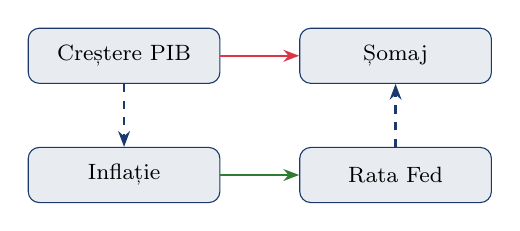
\begin{tikzpicture}[
            node distance=0.5cm,
            box/.style={rectangle, rounded corners, draw=MainBlue, fill=MainBlue!10,
                        text width=2.2cm, minimum height=0.7cm, align=center, font=\footnotesize},
            arrow/.style={-{Stealth[length=2mm]}, thick, MainBlue}
        ]
            \node[box] (gdp) {Creștere PIB};
            \node[box, right=1cm of gdp] (unemp) {Șomaj};
            \node[box, below=0.8cm of gdp] (infl) {Inflație};
            \node[box, right=1cm of infl] (fed) {Rata Fed};

            \draw[arrow, IDAred] (gdp) -- (unemp);
            \draw[arrow, Forest] (infl) -- (fed);
            \draw[arrow, dashed] (gdp) -- (infl);
            \draw[arrow, dashed] (fed) -- (unemp);
        \end{tikzpicture}
    \end{center}

    \vspace{0.3em}
    \begin{columns}[T]
        \begin{column}{0.48\textwidth}
            \textbf{Constatări Cheie:}
            \begin{itemize}
                \item PIB Granger-cauzează șomajul
                \item Inflația Granger-cauzează politica Fed
                \item VAR captează aceste dinamici
            \end{itemize}
        \end{column}
        \begin{column}{0.48\textwidth}
            \textbf{Aplicații Practice:}
            \begin{itemize}
                \item Prognoză economică
                \item Analiză de politici
                \item Managementul riscului în portofolii
            \end{itemize}
        \end{column}
    \end{columns}
\end{frame}

%=============================================================================
% SECTION 6: MODEL SELECTION GUIDE
%=============================================================================
\section{Selecția Modelului: Ghid Practic}

\begin{frame}{Cadrul de Decizie}
    \begin{center}
        \includegraphics[width=0.90\textwidth, height=0.70\textheight, keepaspectratio]{ch10_model_selection_flowchart.pdf}
    \end{center}
\end{frame}

\begin{frame}{Rezumat Selecție Model}
    \begin{table}[h]
        \footnotesize
        \centering
        \begin{tabular}{p{2.5cm}p{3.5cm}p{3.5cm}p{3cm}}
            \toprule
            \textbf{Tip Date} & \textbf{Caracteristici} & \textbf{Model Recomandat} & \textbf{Alternative} \\
            \midrule
            Randamente financiare & Fără trend, clustering vol. & ARIMA-GARCH & EGARCH, GJR \\
            \addlinespace
            Sezonalitate simplă & Trend + o perioadă sezon. & SARIMA & ETS, Prophet \\
            \addlinespace
            Cicluri lungi & Pete solare, cicluri business & AR + Fourier, TBATS & Metode spectrale \\
            \addlinespace
            Rupturi structurale & COVID, schimbări regim & Prophet & ARIMA intervenție \\
            \addlinespace
            Serii multiple & Interdependențe & VAR, VECM & Modele factoriale \\
            \bottomrule
        \end{tabular}
    \end{table}
\end{frame}

\begin{frame}{Metrici de Evaluare a Prognozei}
    \begin{columns}[T]
        \begin{column}{0.48\textwidth}
            \textbf{Metrici pentru Prognoze Punctuale:}

            \vspace{0.3em}
            \textbf{RMSE} (Root Mean Square Error):
            \[
                \sqrt{\frac{1}{n}\sum_{i=1}^{n}(y_i - \hat{y}_i)^2}
            \]

            \textbf{MAE} (Mean Absolute Error):
            \[
                \frac{1}{n}\sum_{i=1}^{n}|y_i - \hat{y}_i|
            \]

            \textbf{MAPE} (Mean Absolute \% Error):
            \[
                \frac{100}{n}\sum_{i=1}^{n}\left|\frac{y_i - \hat{y}_i}{y_i}\right|
            \]
        \end{column}
        \begin{column}{0.48\textwidth}
            \textbf{Când să Folosim Fiecare:}
            \begin{itemize}
                \item \textbf{RMSE}: Penalizează erorile mari
                \item \textbf{MAE}: Robust la outlieri
                \item \textbf{MAPE}: Independent de scală
            \end{itemize}

            \vspace{0.5em}
            \begin{alertblock}{Validare Încrucișată}
                Folosiți întotdeauna CV pentru serii de timp:
                \begin{itemize}
                    \item Fereastră rulantă
                    \item Fereastră expandabilă
                    \item Nu amestecați niciodată!
                \end{itemize}
            \end{alertblock}
        \end{column}
    \end{columns}
\end{frame}

%=============================================================================
% SECTION 6: SUMMARY
%=============================================================================
\section{Rezumat și Concluzii Cheie}

\begin{frame}{Rezumatul Cursului: Setul Complet de Instrumente}
    \begin{columns}[T]
        \begin{column}{0.48\textwidth}
            \textbf{Înțelegerea Datelor}
            \begin{itemize}
                \item Vizualizare mai întâi!
                \item Testați staționaritatea (ADF, KPSS)
                \item Identificați tipare sezoniere
                \item Verificați rupturi structurale
            \end{itemize}

            \vspace{0.5em}
            \textbf{Modele Clasice}
            \begin{itemize}
                \item ARIMA: Date nesezoniere
                \item SARIMA: Sezonalitate simplă
                \item GARCH: Modelarea volatilității
            \end{itemize}
        \end{column}
        \begin{column}{0.48\textwidth}
            \textbf{Abordări Moderne}
            \begin{itemize}
                \item Prophet: Interpretabil, gestionează rupturi
                \item TBATS: Sezonalități multiple/lungi
                \item VAR/VECM: Serii de timp multiple
            \end{itemize}

            \vspace{0.5em}
            \textbf{Cele Mai Bune Practici}
            \begin{itemize}
                \item Verificați întotdeauna diagnosticele
                \item Folosiți validare încrucișată
                \item Comparați modele multiple
                \item Cunoașterea domeniului contează!
            \end{itemize}
        \end{column}
    \end{columns}
\end{frame}

\begin{frame}{Recomandări Finale}
    \begin{enumerate}
        \item \textbf{Începeți Simplu}: Începeți cu vizualizare și statistici de bază
        \item \textbf{Testați Ipotezele}: Staționaritate, normalitate, independență
        \item \textbf{Iterați}: Model $\rightarrow$ Diagnostice $\rightarrow$ Îmbunătățire
        \item \textbf{Comparați}: Nu vă bazați niciodată pe un singur model
        \item \textbf{Validați}: Testarea out-of-sample este esențială
        \item \textbf{Comunicați}: Vizualizări și interpretări clare
    \end{enumerate}

    \vspace{0.5em}
    \begin{exampleblock}{Amintiți-vă}
        ``Toate modelele sunt greșite, dar unele sunt utile.'' --- George Box

        \vspace{0.3em}
        Scopul nu este predicția perfectă, ci perspective utile și prognoze rezonabile.
    \end{exampleblock}
\end{frame}

\begin{frame}{Întrebări?}
    \begin{center}
        \Large\textcolor{MainBlue}{Întrebări?}

        \vspace{1cm}

        \normalsize
        \textbf{Pași Următori:}
        \begin{itemize}
            \item Exersați cu notebook-ul Jupyter
            \item Aplicați aceste metode pe propriile date
            \item Comparați diferite modele pe același set de date
        \end{itemize}

        \vspace{0.5cm}

        Materiale Curs: \texttt{github.com/danpele/Time-Series-Analysis}
    \end{center}
\end{frame}

\end{document}
